\documentclass[11pt]{article}

\usepackage[margin=1in]{geometry}
\usepackage{array}
\usepackage{longtable}
\usepackage{booktabs}
\usepackage{parskip}
\usepackage{enumitem}
\usepackage{url}
\usepackage{graphicx}
\usepackage{amsmath,amssymb}
\usepackage{float}

\setlength{\LTcapwidth}{\textwidth}

% Same look as \titleformat{\section}{\large\bfseries}{}{0em}{} from A1, without needing titlesec
\makeatletter
\renewcommand\section{\@startsection{section}{1}{\z@}{1.2em}{0.5em}{\large\bfseries}}
\renewcommand\subsection{\@startsection{subsection}{2}{\z@}{0.6em}{0.2em}{\normalsize\bfseries}}
\makeatother

% Column types for the tables
\newcolumntype{L}[1]{>{\raggedright\arraybackslash}p{#1}}

\graphicspath{{figures/}}
\newcommand{\code}[1]{\texttt{#1}}

\title{\vspace{-3em}{CSC490 Assignment A3: Pre-training nanochat\vspace{-1em}}}

\author{
  Prithvi Seran (1009973343) \and
  Vraj Shah (1009102695) \and
  Tyseer Toufiq (1009364064) \and
  Joshua Crisologo (1009860438)
}
\date{}

\begin{document}


\maketitle
\vspace{-2.5em}

\section*{Part 1: Architecture Review}

\subsection*{The Original nanochat (October 13, 2025)}

The original nanochat \cite{nanochat} (commit \code{3a5e0bc}) is a decoder-only, pre-norm Transformer \cite{vaswani,gpt2}. Its size is set by the depth $L$ alone: the width is $d = 64L$, each head has 128 dimensions, and the MLP hidden size is $4d$. The d20 model used for the speedrun (Figure~\ref{fig:oct-arch}) has about 561M parameters. Table~\ref{tab:oct} lists its main design choices.

\begin{figure}[H]
  \centering
  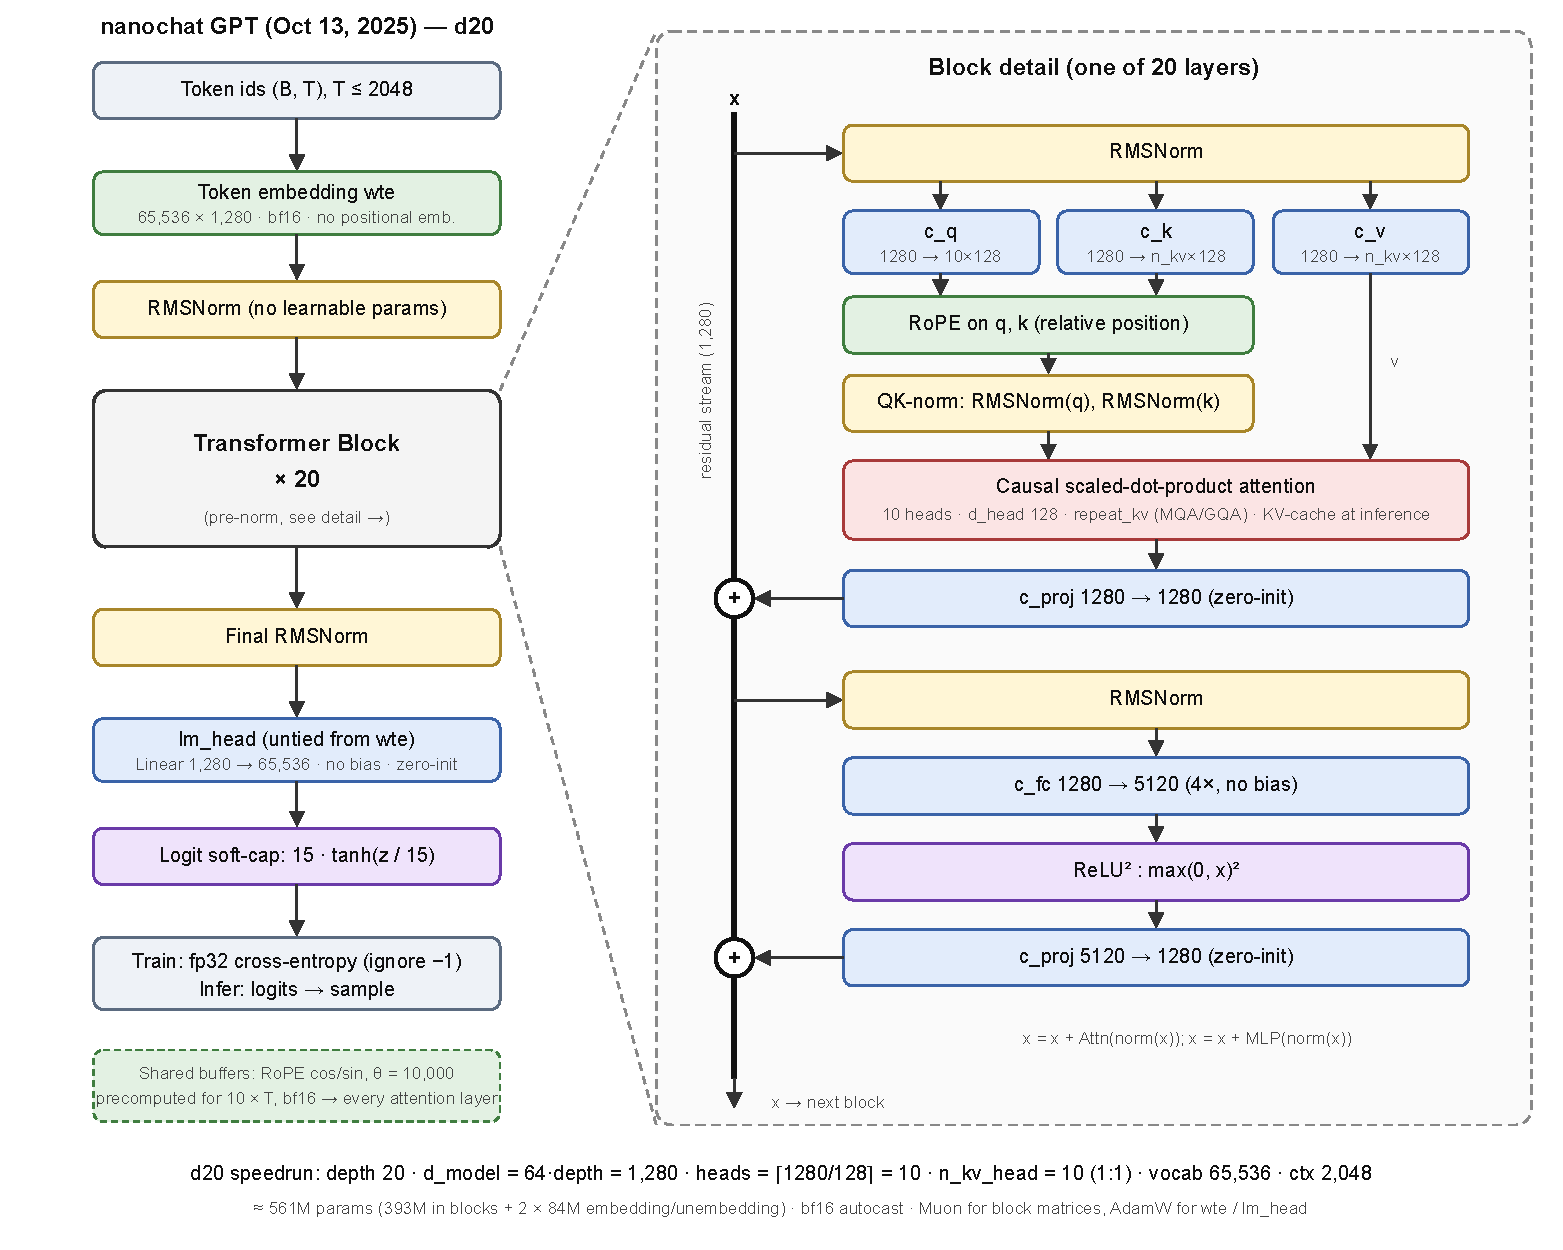
\includegraphics[width=0.9\textwidth]{nanochat_oct_architecture.pdf}
  \caption{The original nanochat architecture (October 13, 2025) at depth 20. Left: the full model. Right: one of the 20 pre-norm Transformer blocks.}
  \label{fig:oct-arch}
\end{figure}

{\small
\renewcommand{\arraystretch}{1.3}
\begin{longtable}{L{2.6cm} L{6.0cm} L{5.6cm}}
\caption{Main architecture choices in the original nanochat.}\label{tab:oct}\\
\toprule
\textbf{Component} & \textbf{Choice} & \textbf{Why} \\
\midrule
\endfirsthead

\toprule
\textbf{Component} & \textbf{Choice} & \textbf{Why} \\
\midrule
\endhead

\bottomrule
\endfoot

\textbf{Position} & RoPE on $q$ and $k$, $\theta = 10{,}000$, all head dims rotated \cite{roformer} & Relative position with no extra parameters \\
\midrule
\textbf{Normalization} & RMSNorm with no learnable gain, pre-norm, also after the embedding \cite{rmsnorm} & Cheaper than LayerNorm and keeps the residual stream stable \\
\midrule
\textbf{Attention} & Causal multi-head attention with QK-norm \cite{qknorm} & QK-norm bounds attention logits at high learning rates \\
\midrule
\textbf{MLP} & $4d$ hidden, ReLU$^2$ activation \cite{primer} & Same cost as GELU and strong in speedruns \\
\midrule
\textbf{Output} & Untied \code{lm\_head}; logit soft-cap $15\tanh(z/15)$ \cite{gemma2} & Separate learning rates; prevents over-confident logits \\
\midrule
\textbf{Other} & No biases; output projections initialized to zero & Simpler; each block starts as the identity \\
\midrule
\textbf{Optimizer} & Muon \cite{muon} for the block matrices, AdamW \cite{adamw} for the embedding and \code{lm\_head} & Muon trains the large matrices faster \\

\end{longtable}
}

\subsection*{Changes in the July 2026 Version}

Our baseline is the July 2026 version (\code{92d63d4}). Most of the changes since October come from the modded-nanogpt speedrun \cite{modded}:
\begin{itemize}[leftmargin=1.2em, itemsep=0em, topsep=0.1em, parsep=0em]
  \item sliding-window attention in an \code{SSSL} pattern, using FlashAttention-3 \cite{fa3};
  \item value embeddings \cite{valueres} and learned per-layer residual scalars;
  \item RoPE $\theta$ raised to 100,000 and a smaller vocabulary of 32,768 tokens;
  \item one combined Muon/AdamW optimizer, now with weight decay.
\end{itemize}
The ReLU$^2$ MLP has not changed, and RoPE is still applied to every head dimension with one $\theta$ for all layers. Our proposed changes target these two parts.

\subsection*{Proposed Changes}

ModernBERT \cite{modernbert} updated BERT \cite{bert} with components from recent LLMs and tested its choices with ablations. July nanochat already has most of them, including bias-free layers, RoPE, pre-norm, alternating local and global attention, and FlashAttention. We take three ideas from ModernBERT that nanochat lacks: the GeGLU MLP, separate RoPE $\theta$ values for local and global layers, and partial RoPE, which ModernBERT tested but did not adopt. Table~\ref{tab:changes} summarizes them and Figure~\ref{fig:changes} shows each one.

\textbf{What we ablate.} Part 2 ablates GeGLU and partial RoPE. At d12 neither changes the parameter count or FLOPs, and each is a single flag, so a gap from the baseline that is larger than seed noise can be attributed to the change. We leave change 3 for Part 4: ModernBERT found no difference between $\theta$ settings during pretraining and only raised the global $\theta$ when it extended its context length. ModernBERT's ablations used encoders of at most 150M parameters, so the results may not carry over to a causal decoder like nanochat.

\begin{figure}[H]
  \centering
  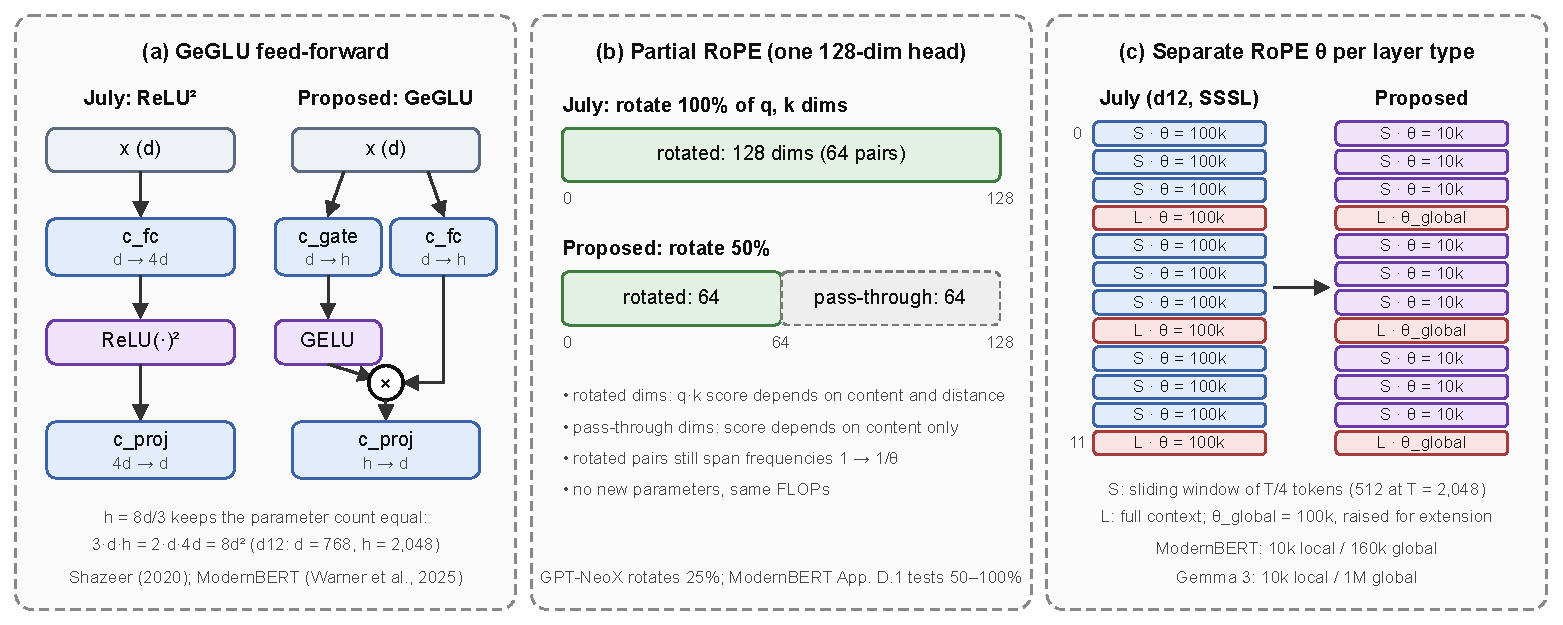
\includegraphics[width=0.85\textwidth]{proposed_changes.pdf}
  \caption{The three proposed changes: (a) GeGLU MLP, (b) partial RoPE, (c) separate RoPE $\theta$ for sliding-window (S) and full-context (L) layers.}
  \label{fig:changes}
\end{figure}

{\small
\renewcommand{\arraystretch}{1.3}
\begin{longtable}{L{2.4cm} L{4.2cm} L{4.2cm} L{3.4cm}}
\caption{Proposed architecture changes relative to July 2026 nanochat ($d$ = model width, $T$ = context length).}\label{tab:changes}\\
\toprule
\textbf{Change} & \textbf{Motivation} & \textbf{Technical Details} & \textbf{Potential Impact} \\
\midrule
\endfirsthead

\toprule
\textbf{Change} & \textbf{Motivation} & \textbf{Technical Details} & \textbf{Potential Impact} \\
\midrule
\endhead

\bottomrule
\endfoot

\textbf{1. GeGLU MLP} \newline \cite{glu} &
In T5, gated MLPs reached lower perplexity than ReLU and GELU MLPs with the same parameter count \cite{glu}. PaLM \cite{palm}, LLaMA \cite{llama} and ModernBERT all use one. &
$W_{\text{proj}}\big(\mathrm{GELU}(W_{\text{gate}}x) \odot W_{\text{fc}}x\big)$ with $h = 8d/3$, so parameters match ReLU$^2$ ($h = 2{,}048$ at d12). Flag \code{-{}-mlp-type=geglu}. &
Same parameters and FLOPs. Expect slightly lower loss. ReLU$^2$ is a strong baseline, so a tie is possible. \\
\midrule

\textbf{2. Partial RoPE} \newline \cite{neox} &
Full RoPE mixes position into every dimension, while unrotated dims can match on content at any distance. GPT-NeoX rotates 25\% of each head \cite{neox}. ModernBERT found 50--75\% slightly better than 100\% but kept 100\% because its ablations ran at a much smaller scale than the final model. &
Rotate the first 64 of the 128 head dims and pass the rest through unchanged. Flag \code{-{}-rope-frac=0.5}. &
No new parameters or FLOPs. Small or no gain at picochat scale; may help context extension. \\
\midrule

\textbf{3. Separate RoPE $\theta$ for local and global layers} \newline \cite{gemma3} &
July uses $\theta = 100{,}000$ everywhere, even in sliding-window layers that only see $T/4$ tokens. ModernBERT uses 10k local and 160k global; Gemma 3 uses 10k and 1M \cite{gemma3}. &
Two cos/sin tables: sliding-window layers use $\theta = 10{,}000$ and full-context layers keep 100,000. Raise only the global $\theta$ when extending context. &
No new parameters or FLOPs. We expect no effect at a fixed context length; any benefit should appear during context extension. \\

\end{longtable}
}

\newpage

\section*{Part 2: Ablations on a Nano Nanochat}

\subsection*{Results}

We tracked every run in the team's Weights \& Biases (W\&B) project:
\begin{center}
\small\url{https://forge.coreweave.com/wandb/vraj-shah2121-university-of-toronto/nanochat/workspace}
\end{center}
The three full runs are \code{d12\_baseline}, \code{d12\_geglu} and \code{d12\_rope50}. Each logged validation bits per byte (BPB) every 250 steps, training loss, throughput and MFU every 100 steps, and the CORE score at steps 2000 and 2520. CORE was capped at 500 examples per task. Table~\ref{tab:part2-results} summarizes the runs, and Figure~\ref{fig:part2-training} compares their training curves.

The W\&B configs differ only in the flag under test (\code{--mlp-type=geglu} or \code{--rope-frac=0.5}) and the run name. All three runs use seed 42 and 2,520 steps, with the same estimated total of $1.0 \times 10^{18}$ FLOPs. All three start from a validation BPB of 3.16867, because the zero-initialized output projections make the changes invisible at step 0.

\begin{table}[H]
\centering
\caption{Picochat (d12) ablation results. For validation BPB, lower is better; for CORE, higher is better. Gaps are relative to the baseline. Throughput and MFU are medians of the logged steps after the first five.}
\label{tab:part2-results}
\begin{tabular}{@{}lrrr@{}}
\toprule
 & Baseline & GeGLU & Partial RoPE (50\%) \\
\midrule
Hardware & $8 \times$ H200 & $8 \times$ H200 & $8 \times$ H100 \\
Final validation BPB & 0.84537 & 0.84754 & 0.84505 \\
\quad Gap to baseline & -- & $+0.00217$ & $-0.00031$ \\
\quad Gap (\%) & -- & $+0.26\%$ & $-0.04\%$ \\
CORE at step 2000 & 0.1570 & 0.1547 & 0.1589 \\
Final CORE (step 2520) & 0.1734 & 0.1656 & 0.1705 \\
\quad Gap to baseline & -- & $-0.0078$ & $-0.0029$ \\
\quad Tasks better / worse (of 22) & -- & 9 / 13 & 8 / 13 \\
Training time (min) & 5.23 & 5.45 & 5.41 \\
Throughput (million tokens/s) & 4.33 & 4.16 & 4.10 \\
MFU (\%) & 41.6 & 39.9 & 39.4 \\
\bottomrule
\end{tabular}
\end{table}

\begin{figure}[H]
\centering
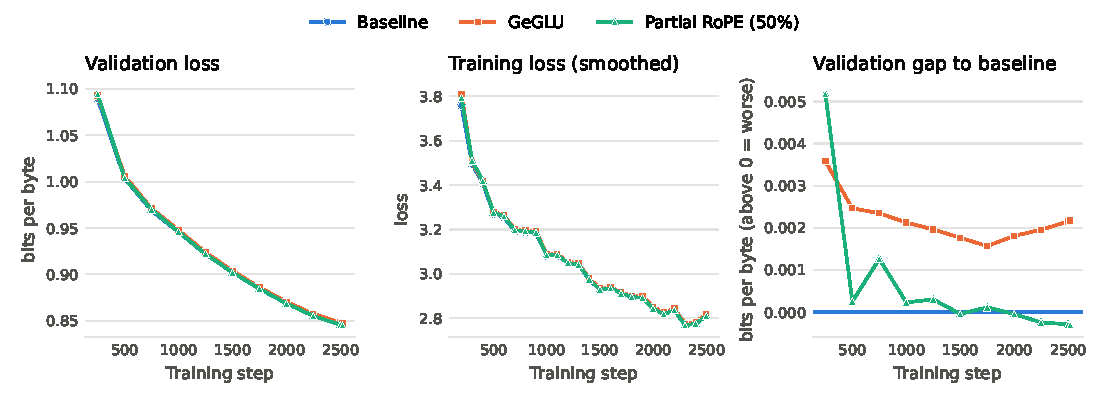
\includegraphics[width=\textwidth]{part2_training.pdf}
\caption{Training curves from the W\&B runs. The validation and training curves almost overlap, so the right panel plots each change's validation gap to the baseline. The plots start after the steep early drop (step 250 for validation, step 200 for training loss).}
\label{fig:part2-training}
\end{figure}

\subsection*{Impact of Each Change}

\textbf{Overall.} Neither change clearly improved the model at this scale, which fits the small or null effect we predicted in Part 1. Figure~\ref{fig:part2-core} shows why the CORE gaps are weak evidence: individual tasks move by as much as 0.10, in both directions. The standard error of the mean gap across tasks is about 0.008, so GeGLU's gap is 0.95 standard errors from zero and partial RoPE's is 0.34.

\textbf{GeGLU.} GeGLU has a slightly worse validation BPB than the baseline at all 11 evaluations after step 0, with a gap between 0.0016 and 0.0036 that had not closed by the end of training. Its CORE score is also lower, though within the task-level noise above. These evaluations come from one training run and are correlated, so the consistent sign is not 11 independent results. On the same GPU model as the baseline, GeGLU ran about 4\% slower in both throughput and training time. Its parameter count and estimated FLOPs match the baseline, so this slowdown is not captured by the FLOP estimate. We do not see the gain reported for gated MLPs in the literature \cite{glu}, but this run cannot rule one out: it is short and small, and it has only one seed.

\textbf{Partial RoPE (50\%).} We cannot distinguish partial RoPE from the baseline. It trails early (a BPB gap of $+0.0052$ at step 250), catches up by about step 1500, and finishes $0.00031$ ahead. It also led on CORE at step 2000 ($+0.0019$) but trailed at step 2520 ($-0.0029$), and that change of sign suggests the gap is mostly noise. ModernBERT reported a slight gain at 50--75\% \cite{modernbert}, and we neither confirm nor contradict that here. We also cannot read its throughput as a cost of the change: this run used H100s while the baseline used H200s, and the change rotates fewer dimensions, so it should not add work.

\textbf{Limitations.} We trained one model per configuration, so we have no direct measure of seed noise. The closest evidence is two identical 100-step smoke tests with the same seed, whose validation BPB differed by 0.00014. That shows only that runs are not fully deterministic, and it is a lower bound on noise, since changing the seed should vary results more. The GeGLU gap is about 15 times that figure and the partial RoPE gap about 2 times. The hardware also differs across runs, as noted above. It should not affect the loss curves much, but it does limit the throughput comparison to baseline versus GeGLU.

\begin{figure}[H]
\centering
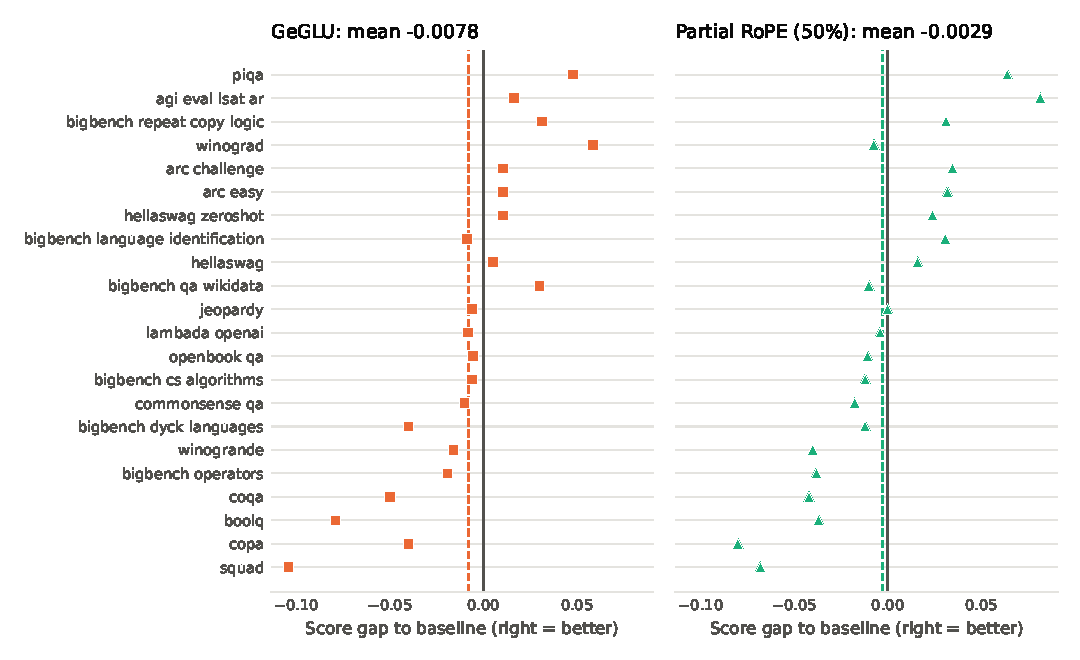
\includegraphics[width=0.9\textwidth]{part2_core_tasks.pdf}
\caption{Final CORE gap to the baseline on each of the 22 tasks. The solid line marks zero and the dashed line marks the mean gap. Tasks are sorted by their average gap across the two changes. Both changes gain on some tasks and lose on others.}
\label{fig:part2-core}
\end{figure}

\newpage

\section*{Part 3: Hardware Efficiency Curves}

\newpage

\section*{Part 4: Extending the Context Window}

\newpage

\section*{Part 5: Training Our Final Nanochat}

\subsection*{Final Model Configuration}

Table~\ref{tab:final-config} gives the data, architecture and hardware configuration of our final nanochat and why we chose it. Most of the justification comes from our picochat runs in Parts 2 and 4, and several choices keep the final model directly comparable with the d12 picochat.

{\small
\renewcommand{\arraystretch}{1.3}
\begin{longtable}{L{2.6cm} L{4.0cm} L{7.8cm}}
\caption{Final nanochat configuration.}\label{tab:final-config}\\
\toprule
\textbf{Configuration} & \textbf{Choice} & \textbf{Justification} \\
\midrule
\endfirsthead

\toprule
\textbf{Configuration} & \textbf{Choice} & \textbf{Justification} \\
\midrule
\endhead

\bottomrule
\endfoot

\textbf{Data} &
ClimbMix with the same 32,768-token tokenizer as the picochat; 12 tokens per parameter (about 5.2B tokens); 2,048-token context throughout &
Same data and tokenizer as the picochat, so the two models compare directly. 12 tokens per parameter is the compute-optimal ratio nanochat measured for its own architecture, and our picochat used the same ratio. We read ``the full pre-training dataset'' as this full compute-optimal budget, since all 400B tokens would take about 77 times the compute. In Part 4, training at 512 tokens first lowered CORE (0.162 vs 0.173) for only about a 7\% speedup. \\
\midrule

\textbf{Architecture} &
d20 (20 layers, width 1,280) with partial RoPE (50\%) &
d20 is the original nanochat size and needs about 15 times the picochat's compute. In Part 2, partial RoPE matched the baseline (validation BPB 0.84505 vs 0.84537) at no extra cost, while GeGLU was worse on both loss and CORE, so we leave GeGLU out. We did not implement separate RoPE $\theta$ values. \\
\midrule

\textbf{Hardware} &
8 $\times$ H200 in bf16 &
A 20-step smoke test of d20 on 8 H200s peaked at about 72 GiB per GPU (d12 used 27 GiB). That would leave under 8 GiB of headroom on an 80 GB H100, while the H200's 141 GB runs the full batch with room to spare. The smoke test also reached 48\% MFU, above the 41.6\% of our d12 runs, and the H200 matches the picochat baseline's hardware and precision. \\

\end{longtable}
}

\textbf{Training.} We launched the run through our Modal script with \code{--depth=20 --rope-frac=0.5}, saving a checkpoint every 1,000 steps, and left every other setting at its default. nanochat's batch-size rule chose about 1M tokens per step for d20, twice the d12 batch, and raised the learning rates by $\sqrt{2}$ to match. Our first attempt stopped at step 1,920 of 4,980, most likely when the Modal client on our laptop shut down, and it had saved no checkpoint. We relaunched it to run independently of the laptop, which is why we added checkpoints. The completed run trained for 4,980 steps on 5.22B tokens ($1.51 \times 10^{19}$ FLOPs) in 64.7 minutes, at 1.34M tokens per second and 49.0\% MFU. The job cost \$52.08 in Modal credits, including startup and evaluation. Together with the failed attempt, the smoke test and the scaling-law runs below, Part 5 used about \$97. The final model reached a validation BPB of 0.7367 and a CORE score of 0.242, compared with 0.8454 and 0.173 for the d12 baseline. The full CORE evaluation over every example, instead of 500 per task, gives 0.239, close to the 0.257 of GPT-2 (1.6B) \cite{nanochat}.

\subsection*{Scaling Law: Predicted vs Actual}

To predict the nanochat's loss from cheap runs, we trained three more picochats (d8, d10 and d14) with the same recipe as the final model: partial RoPE, 12 tokens per scaling parameter, ClimbMix and the same tokenizer. Together with the d12 partial RoPE run from Part 2, they span a 15-fold range of compute (Table~\ref{tab:part5-points}). Our eval dataset is ClimbMix's held-out validation shard: every run reports its BPB on the same 42M validation tokens at the end of training. Following Kaplan et al.\ \cite{kaplan} and Hoffmann et al.\ \cite{chinchilla}, we model the loss as a power law in training compute, $\text{BPB} = a\,C^{-b}$, which is a straight line in log-log space, and fit it by least squares to the four picochats only.

\begin{table}[H]
\centering
\caption{Runs used for the scaling law. All use partial RoPE and 12 tokens per scaling parameter. The d20 was not used in the fit. Training times are on 8 H200s, except d12, which ran on 8 H100s in Part 2.}
\label{tab:part5-points}
\begin{tabular}{@{}lrrrrrr@{}}
\toprule
Model & Scaling params & Tokens & FLOPs & Val BPB & CORE & Train time \\
\midrule
d8  & 41.9M  & 0.50B & $1.49 \times 10^{17}$ & 0.9416 & 0.105 & 1.4 min \\
d10 & 70.1M  & 0.84B & $4.17 \times 10^{17}$ & 0.8926 & 0.122 & 2.3 min \\
d12 & 110.1M & 1.32B & $1.00 \times 10^{18}$ & 0.8451 & 0.171 & 5.4 min \\
d14 & 164.2M & 1.97B & $2.22 \times 10^{18}$ & 0.8095 & 0.181 & 10.8 min \\
\midrule
d20 (predicted) & & & & 0.7265 & & \\
d20 (actual) & 435.2M & 5.22B & $1.51 \times 10^{19}$ & 0.7367 & 0.242 & 64.7 min \\
\bottomrule
\end{tabular}
\end{table}

The fit is $\text{BPB} = 8.80\,C^{-0.0565}$. It matches the picochats closely ($R^2 = 0.999$ in log space), with every point within 0.33\% of the line. At the d20's $1.51 \times 10^{19}$ FLOPs it predicts a validation BPB of 0.7265, and refitting with each picochat left out in turn gives predictions between 0.7230 and 0.7278. The d20 reached 0.7367, 1.4\% worse than predicted and just outside that range (Figure~\ref{fig:part5-scaling}).

\begin{figure}[H]
\centering
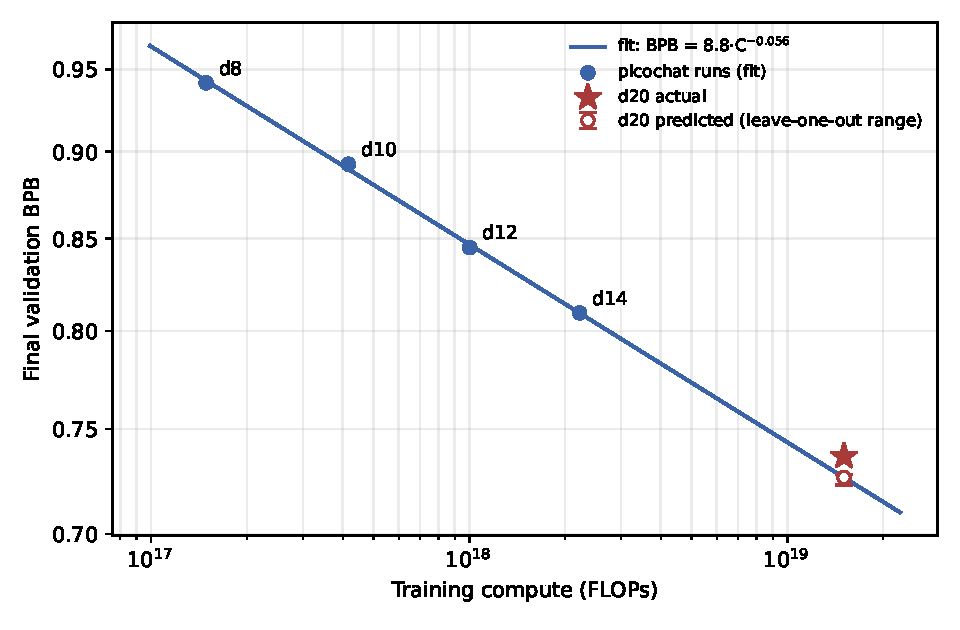
\includegraphics[width=0.75\textwidth]{part5_scaling.pdf}
\caption{Validation BPB against training compute. The line is fitted to the four picochats; the open circle is its d20 prediction, with the range from leave-one-out refits, and the star is the actual d20.}
\label{fig:part5-scaling}
\end{figure}

The prediction was close but optimistic, and we see three reasons. First, a pure power law assumes the loss keeps falling at the same rate, while real scaling curves bend toward an irreducible loss. Hoffmann et al.\ model this with a constant term, $L = E + A\,C^{-\alpha}$ \cite{chinchilla}, but four points are too few to fit that extra parameter reliably, so our line is likely too steep at large compute. Second, the d20 is 6.8 times beyond our largest fitted model, so a small error in the slope grows over the extrapolation. Third, the recipe is not perfectly constant across sizes: nanochat's batch-size rule gave d8 262K tokens per step, d10 to d14 524K and d20 1M, with matching learning-rate changes. In absolute terms the error is small, 0.010 BPB against the 0.073 BPB the model gained from d14 to d20.

CORE does not follow a power law, but over these runs it grew roughly linearly in log compute. A straight-line fit of CORE against $\log_{10} C$ on the four picochats predicts 0.244 for the d20, close to the 0.242 it reached.

\subsection*{Results}

Table~\ref{tab:part5-results} compares the final nanochat with the two d12 picochats from Part 2.

\begin{table}[H]
\centering
\caption{Picochat and nanochat results. CORE uses 500 examples per task, as in Part 2. Prompts correct is the number of our 99 completion prompts answered correctly (see Emergent Abilities).}
\label{tab:part5-results}
\small
\begin{tabular}{@{}lrrr@{}}
\toprule
 & Picochat (baseline) & Picochat (partial RoPE) & Nanochat (partial RoPE) \\
\midrule
Depth / width & d12 / 768 & d12 / 768 & d20 / 1,280 \\
Scaling parameters & 110.1M & 110.1M & 435.2M \\
Training tokens & 1.32B & 1.32B & 5.22B \\
Training FLOPs & $1.00 \times 10^{18}$ & $1.00 \times 10^{18}$ & $1.51 \times 10^{19}$ \\
Hardware & $8 \times$ H200 & $8 \times$ H100 & $8 \times$ H200 \\
Batch size (tokens) & 524K & 524K & 1.05M \\
Training time (min) & 5.2 & 5.4 & 64.7 \\
MFU (\%) & 41.6 & 39.4 & 49.0 \\
Final validation BPB & 0.8454 & 0.8451 & 0.7367 \\
Final CORE & 0.173 & 0.171 & 0.242 \\
Prompts correct (of 99) & -- & 50 & 74 \\
\bottomrule
\end{tabular}
\end{table}

\textbf{Scale.} Going from d12 to d20 multiplied training compute by 15 and is by far the largest change. Validation BPB fell by 12.8\% (0.845 to 0.737), CORE rose by 0.07 (0.171 to 0.242), and the model answered 24 more of our prompts correctly. The larger model also used the GPUs better: MFU rose from about 40\% to 49\%, because the bigger matrix multiplications keep the H200s busier.

\textbf{Partial RoPE.} We kept partial RoPE because it matched the baseline at d12 in Part 2. We did not train a d20 baseline, which would have cost another \$52, so we cannot measure its effect at d20 directly. The d20 landed 1.4\% above the trend fitted to partial RoPE picochats, which gives no sign that partial RoPE helps more at larger scale, but we cannot separate this from the extrapolation error discussed above.

\textbf{Excluded changes.} We left out GeGLU, which was slightly worse at d12, and the short-context recipe from Part 4, which lowered CORE. Neither is part of the final model, so the nanochat's gains come from scale under the July architecture with partial RoPE.

\subsection*{Emergent Abilities}

Wei et al.\ call an ability emergent if it is absent in smaller models but present in larger ones \cite{wei-emergent}. To look for such abilities, we gave the d12 partial RoPE picochat and the d20 nanochat the same 99 short completion prompts covering geography, science, history, language and arithmetic. Both are base models without chat finetuning, so each prompt is the start of a sentence (for example ``The capital of Japan is''), and each model completes it with greedy decoding for 12 tokens. A script marks a completion correct if an accepted answer appears in its first six words, and we then read every completion to remove false matches. The picochat answered 50 prompts correctly and the nanochat 74. The nanochat was right and the picochat wrong on 25 prompts; the reverse happened once. Table~\ref{tab:emergent} lists 10 of the 25.

{\small
\renewcommand{\arraystretch}{1.3}
\begin{longtable}{L{5.4cm} L{4.6cm} L{4.4cm}}
\caption{Ten prompts the nanochat answers correctly and the picochat does not (greedy completions, trimmed).}\label{tab:emergent}\\
\toprule
\textbf{Prompt} & \textbf{Picochat (d12)} & \textbf{Nanochat (d20)} \\
\midrule
\endfirsthead

\toprule
\textbf{Prompt} & \textbf{Picochat (d12)} & \textbf{Nanochat (d20)} \\
\midrule
\endhead

\bottomrule
\endfoot

1. The capital of Japan is & Hokkaido, which is the capital of the & Tokyo. \\
2. The capital of India is & Karnataka, which is the capital of the country & New Delhi. \\
3. The Mona Lisa was painted by & the French artist Pierre de Coubertin in 17 & Leonardo da Vinci in 1503. \\
4. The freezing point of water in degrees Celsius is & 32 degrees Celsius. & 0 degrees Celsius. \\
5. The powerhouse of the cell is the & nucleus. & mitochondria. \\
6. The hardest natural substance on Earth is & water. & diamond. \\
7. The first person to walk on the Moon was & a man named Apollo 11, who was born in & Neil Armstrong, who walked on the Moon on July \\
8. The telephone was invented by & the French in 1860 & Alexander Graham Bell in 1876. \\
9. The plural of mouse is & mouse. & mice. \\
10. The main language spoken in Brazil is & the native language of the country. & Portuguese. \\

\end{longtable}
}

Most of the nanochat's new abilities are factual recall: capitals, scientists, inventors and basic science facts that the picochat gets wrong or avoids. Both models still fail every arithmetic prompt (the nanochat completes ``7 + 5 ='' with 10), and the nanochat still makes factual errors, such as naming Sydney as the capital of Australia. The one prompt only the picochat got right was the name of Martin Luther King Jr.'s ``I Have a Dream'' speech.

We would not call these abilities emergent in the strong sense of a sudden jump. CORE rose steadily with compute and fell on the line predicted from the picochats, so the nanochat's gains look like the continuation of a smooth trend. This fits Schaeffer et al.\ \cite{schaeffer-mirage}, who argue that many reported emergent abilities come from all-or-nothing metrics: a question scored right or wrong appears to switch on at some scale even when the probability of the right answer grows smoothly. Our per-prompt checks are exactly such all-or-nothing tests.

\newpage
\begin{thebibliography}{99}

\bibitem{nanochat}
A. Karpathy, ``nanochat: A tiny chatbot arena and training harness,'' GitHub, 2025. \url{https://github.com/karpathy/nanochat/discussions/481}

\bibitem{vaswani}
A. Vaswani et al., ``Attention Is All You Need,'' \textit{NeurIPS}, 2017. arXiv:1706.03762.

\bibitem{gpt2}
A. Radford et al., ``Language Models are Unsupervised Multitask Learners,'' OpenAI technical report, 2019.

\bibitem{roformer}
J. Su et al., ``RoFormer: Enhanced Transformer with Rotary Position Embedding,'' \textit{Neurocomputing}, vol.~568, 2024. arXiv:2104.09864.

\bibitem{rmsnorm}
B. Zhang and R. Sennrich, ``Root Mean Square Layer Normalization,'' \textit{NeurIPS}, 2019. arXiv:1910.07467.

\bibitem{qknorm}
A. Henry et al., ``Query-Key Normalization for Transformers,'' \textit{Findings of EMNLP}, 2020. arXiv:2010.04245.

\bibitem{primer}
D. R. So et al., ``Primer: Searching for Efficient Transformers for Language Modeling,'' \textit{NeurIPS}, 2021. arXiv:2109.08668.

\bibitem{gemma2}
Gemma Team, ``Gemma 2: Improving Open Language Models at a Practical Size,'' arXiv:2408.00118, 2024.

\bibitem{muon}
K. Jordan et al., ``Muon: An optimizer for hidden layers in neural networks,'' 2024. \url{https://kellerjordan.github.io/posts/muon/}

\bibitem{adamw}
I. Loshchilov and F. Hutter, ``Decoupled Weight Decay Regularization,'' \textit{ICLR}, 2019. arXiv:1711.05101.

\bibitem{modded}
K. Jordan et al., ``modded-nanogpt: Speedrunning the NanoGPT baseline,'' GitHub, 2024. \url{https://github.com/KellerJordan/modded-nanogpt}

\bibitem{fa3}
J. Shah et al., ``FlashAttention-3: Fast and Accurate Attention with Asynchrony and Low-precision,'' arXiv:2407.08608, 2024.

\bibitem{valueres}
Z. Zhou et al., ``Value Residual Learning For Alleviating Attention Concentration In Transformers,'' arXiv:2410.17897, 2024.

\bibitem{modernbert}
B. Warner et al., ``Smarter, Better, Faster, Longer: A Modern Bidirectional Encoder for Fast, Memory Efficient, and Long Context Finetuning and Inference,'' \textit{ACL}, pp.~2526--2547, 2025. \url{https://aclanthology.org/2025.acl-long.127/}

\bibitem{bert}
J. Devlin et al., ``BERT: Pre-training of Deep Bidirectional Transformers for Language Understanding,'' arXiv:1810.04805, 2018.

\bibitem{glu}
N. Shazeer, ``GLU Variants Improve Transformer,'' arXiv:2002.05202, 2020.

\bibitem{palm}
A. Chowdhery et al., ``PaLM: Scaling Language Modeling with Pathways,'' \textit{JMLR}, vol.~24, 2023. arXiv:2204.02311.

\bibitem{llama}
H. Touvron et al., ``LLaMA: Open and Efficient Foundation Language Models,'' arXiv:2302.13971, 2023.

\bibitem{neox}
S. Black et al., ``GPT-NeoX-20B: An Open-Source Autoregressive Language Model,'' \textit{BigScience Workshop on Challenges \& Perspectives in Creating Large Language Models}, 2022. arXiv:2204.06745.

\bibitem{gemma3}
Gemma Team, ``Gemma 3 Technical Report,'' arXiv:2503.19786, 2025.

\bibitem{kaplan}
J. Kaplan et al., ``Scaling Laws for Neural Language Models,'' arXiv:2001.08361, 2020.

\bibitem{chinchilla}
J. Hoffmann et al., ``Training Compute-Optimal Large Language Models,'' \textit{NeurIPS}, 2022. arXiv:2203.15556.

\bibitem{wei-emergent}
J. Wei et al., ``Emergent Abilities of Large Language Models,'' \textit{Transactions on Machine Learning Research}, 2022. arXiv:2206.07682.

\bibitem{schaeffer-mirage}
R. Schaeffer, B. Miranda, and S. Koyejo, ``Are Emergent Abilities of Large Language Models a Mirage?,'' \textit{NeurIPS}, 2023. arXiv:2304.15004.

\end{thebibliography}

\end{document}
